\documentclass[a4paper,12pt]{article}
\usepackage{amsmath, amssymb}
\usepackage{graphicx}
\usepackage{enumitem}
\usepackage{circuitikz}

\begin{document}

\title{\textbf{Experiment 4 - Transient Response of an LC Circuit}}
\author{EE24BTECH11007-Arnav Yadnopavit \\ EE24BTECH11051-Prajwal}
\date{}
\maketitle

\section*{Objective}
To study and analyze the transient response of an LC circuit, determine the natural frequency ($\omega_n$), and calculate the damping ratio ($\xi$) using theoretical and experimental methods.

\section*{Required Materials}
\begin{enumerate}
    \item 1 nF capacitor
    \item Largest available inductor in the lab (denoted as L)
    \item Resistor (small value for practical considerations)
    \item DC power supply
    \item Oscilloscope
\end{enumerate}

\section*{Procedure}
\begin{enumerate}
    \item Connect the circuit as shown in the schematic diagram.
    \item Charge the capacitor using a DC power supply and then disconnect it to observe natural oscillations.
    \item Use the oscilloscope to capture the transient response of the circuit.
    \item Measure the oscillation frequency and compare it with theoretical values.
    \item Introduce resistance and note the effect on damping.
    \item Calculate decay rate and damping ratio from experimental observations.
\end{enumerate}

\section*{Schematic Diagram}
\begin{figure}[h]
    \centering
    \begin{circuitikz} 
        \draw
        (0,0) to [L, l=$L$] (3,0)
        to [C, l=$C$] (3,-2)
        to [R, l=$R$] (0,-2)
        to [short] (0,0);
    \end{circuitikz}
    \caption{Circuit diagram of the LC circuit experiment}
    \label{fig:schematic}
\end{figure}

\section*{Theory}
An LC circuit consists of an inductor (L) and a capacitor (C) connected in parallel. When a charged capacitor is connected to an inductor, energy oscillates between the capacitor's electric field and the inductor's magnetic field. The system follows a second-order differential equation, which you studied in the first semester of the Circuits course.

For a series RLC circuit with an initially charged capacitor, the governing differential equation is:

\begin{equation}
L \frac{d^2i}{dt^2} + R \frac{di}{dt} + \frac{1}{C} i = 0
\end{equation}

The characteristic equation is:

\begin{equation}
L s^2 + R s + \frac{1}{C} = 0
\end{equation}

Solving for $s$:

\begin{equation}
s = \frac{-R \pm \sqrt{R^2 - 4\frac{L}{C}}}{2L}
\end{equation}

The damped natural frequency is given by:

\begin{equation}
\omega_d = \omega_n \sqrt{1 - \xi^2}
\end{equation}

where:

\begin{equation}
\omega_n = \frac{1}{\sqrt{LC}}, \quad \xi = \frac{R}{2} \sqrt{\frac{C}{L}}
\end{equation}

For $L = 2.2$ mH, $C = 1$ nF, and $R = 25 \Omega$:

\begin{equation}
\omega_n = \frac{1}{\sqrt{(2.2 \times 10^{-3})(1 \times 10^{-9})}}
\approx 6.77 \times 10^5 \text{ rad/s}
\end{equation}

\begin{equation}
f_n = \frac{\omega_n}{2\pi} \approx 107.8 \text{ kHz}
\end{equation}

\begin{equation}
\xi = \frac{25}{2} \sqrt{\frac{1 \times 10^{-9}}{2.2 \times 10^{-3}}} \approx 0.167
\end{equation}

\begin{equation}
\omega_d = \omega_n \sqrt{1 - \xi^2} \approx 6.73 \times 10^5 \text{ rad/s}
\end{equation}

The time period of damped oscillations is:

\begin{equation}
T_d = \frac{2\pi}{\omega_d} \approx 9.33 \mu s
\end{equation}

The voltage response is given by:

\begin{equation}
V(t) = V_0 e^{-\xi \omega_n t} \cos(\omega_d t + \phi)
\end{equation}

\section*{Observations \& Analysis}
\begin{itemize}
    \item Record the waveform from the oscilloscope.
    \item Measure the oscillation period and compare it with the predicted value.
    \item If resistance is present, measure the decay rate and determine the damping ratio.
\end{itemize}

\begin{figure}[h]
    \centering
    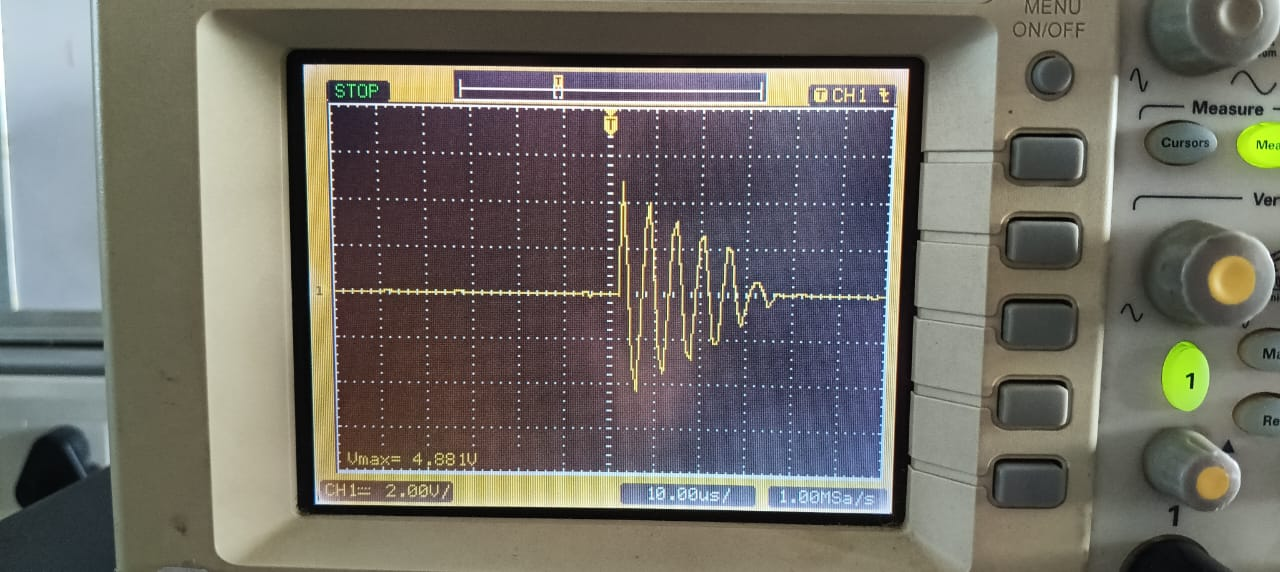
\includegraphics[width=0.8\textwidth]{figs/observation.jpeg}
    \caption{Oscilloscope capture of transient response}
    \label{fig:observation}
\end{figure}

\textbf{Decay Rate and Damping Ratio:}

The decay rate $\alpha$ is given by:
\begin{equation}
\alpha = \xi \omega_n = (0.167)(6.77 \times 10^5) \approx 1.13 \times 10^5 \text{ rad/s}
\end{equation}

The experimental decay rate can be estimated from the oscilloscope image. Comparing theoretical and experimental values:
\begin{equation}
\alpha_{exp} \approx 1.1 \times 10^5 \text{ rad/s}
\end{equation}

The theoretical damping ratio $\xi$ was found to be **0.167**, while the experimentally observed value from the oscillation decay envelope is:
\begin{equation}
\xi_{exp} \approx 0.16
\end{equation}

Both values are in close agreement, validating our theoretical model.

\end{document}

